\chapter{Signal Chain%
  \label{chap:\currfilebase}}


In commercial \ac{EMA}-systems the signal is transmitted
\section{Signal Conditioning}


\subsection{Excitation}

\subsection{Amplification}



\subsection{Filtering}

Whenever we measure a signal in the real world, it will inherently contain some form of noise. Filtering enables us to cut off contributions to the signal amplitude, that are outside the expected signal frequency bandwidth.

The two main types of filters are analog and digital ones, where the digital filters are more versatile, cost-effective and precise compared to their counterpart. Nevertheless, analog filters are required when filtering analog signals, i.e.\ whenever the signal must be denoised or bandwidth limited. As an example, it is advantageous if a signal is denoised, before it is amplified because we do not want to amplify the noise components of the signal. Furthermore electric devices in the signal chain have a bandwidth limited range of operation. Disturbances of the signal occur due to frequency dependant phase shifts or damping when operating outside these ranges. Namely when digitizing a signal, the additional effect of aliasing may disturb a signal significally if it contains frequency components above the Nyquist frequency.

\subsection{Analog to Digital Conversion}

Additionally to other noise sources in the signal chain the \ac{ADC} shows internal noise that can categorized into two uncorrelated main sources. The quantization noise and the thermal noise. The total internal noise can thus be expressed as the Euclidean norm of these two sources.

\begin{align}
  n_\text{ADC} &= \sqrt{n_{\text{ADC},\text{Thermal}}^2 + n_{\text{ADC},\text{Quantization}}^2}
\end{align}

Quantization noise is present due to the process of mapping an infinite number of possible electrical signal values in an analog signal to a finite number of digital codes. Subsequently, any digital output corresponds to an infinite number of analog inputs within range of the output value, plus and minus half the \ac{LSB} size, $s_\text{LBS}$. One can decrease quantization noise by choosing a higher resolution \ac{ADC}.

\begin{align}
  s_\text{LBS} &= \frac{U_{FSR}}{2^m}
\end{align}
where
\begin{description}[topsep=0ex, noitemsep]
  \item $U_{\text{FSR}}$ is the full-scale range of the analog input value and
  \item $m$ is the resolution in number of bits
\end{description}

\begin{figure}[!htb]
  \centering
  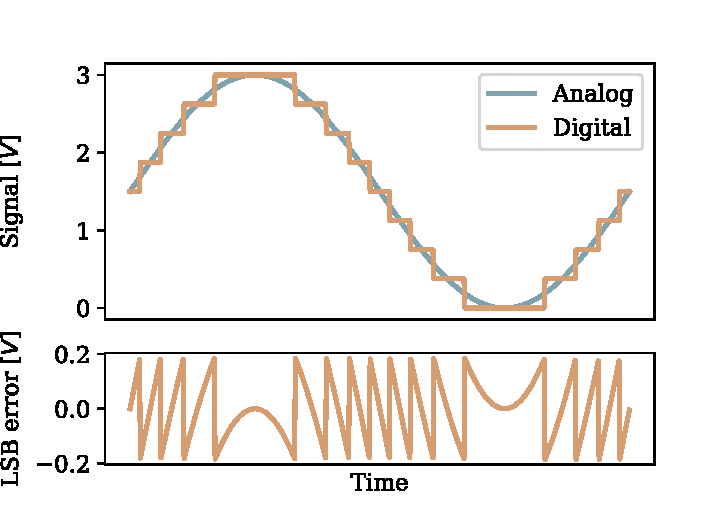
\includegraphics[scale=0.72]{figures/electronics/adc/plot_lsberr}
  \caption[ADC LSB waveform]{\ac{ADC} --- Analog input, digital output and \ac{LSB} error waveform with $s_\text{LBS} = \SI{375}{\milli\volt}$\cite{hall2020fund}%
    \label{fig:plot_lsberr}}
\end{figure}

Thermal noise is a phenomenon inherent in all electrical components. Because of this it is a function of the device design and cannot be affected by the embedded system designer. Typically, one assumes the thermal noise to have a Gaussian distribution.

\begin{figure}
  \centering
  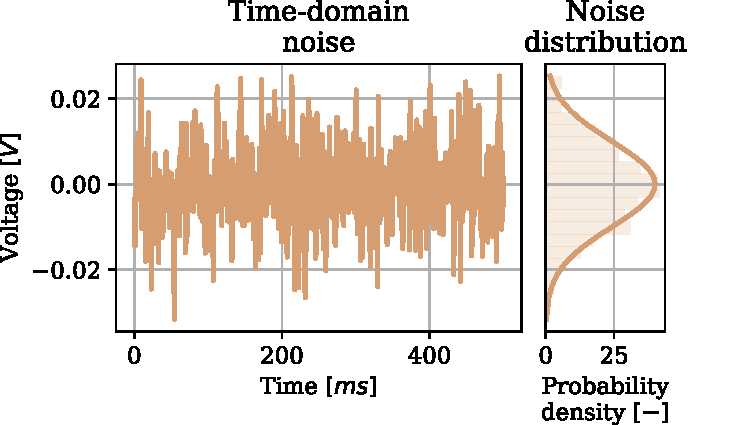
\includegraphics[scale=0.72]{figures/electronics/adc/plot_thermerr}
  \caption[ADC thermal noise]{ADC --- Thermal noise in the time domain with Gaussian probability density~\cite{hall2020fund}%
    \label{fig:plot_themerr}}
\end{figure}
